\section{Introduction}

April 27th, 2010 - Philadelphia Convention Center (Main Hall):  The robot handlers Daniel M. Lofaro and Robert Ellenberg were preparing Jaemi Hubo (the adult-size humanoid robot) for a demonstration for the \textit{Arts and Science Council} of Philadelphia.  During the dress rehearsal one of Jaemi's actuators failed during a demonstration of active balancing and she fell off of a 4 foot high stage.  The results of the impact can be found in Fig.~\ref{fig:fall} and on YouTube\footnote{Jaemi Hubo Fall: http://www.youtube.com/watch?v=DF8zAM4FLB4}\label{link:fall}.  This annual event was a high profile fund raiser for the arts and science programs through the greater Philadelphia area covered widely in the news print, radio, and television.  If this failure would have occurred during the actual event the aftermath would have been even more devastating.  In order for outreach like this event to continue methods to detecting a failure state and using proper mitigation to move to a proper running state must be implemented before proceeding further.  

This work proposes ways to \textbf{detect} when entering a failure state and ways of \textbf{mitigating} such failures.  The adult-size humanoid robot Jaemi Hubo is the primary test platform for this proposed work.  All methods used are written in a broad scope so it can be applicable to other electro mechanical systems.



%On April 27th, 2010: Jaemi Hubo was schedule to be apart of the \textit{Arts and Science Council} annual awards ceremony at the Philadelphia Convention Center.  During the dress rehearsal one of Jaemi's actuators failed ans she fell off of a 1.2 meter stage.

Electro-mechanical systems inevitably fail during use.  Failures during operation typically cause system halts.  This is particularly hazardous to robots that require feedback to balance such as biped humanoid robots.  For biped humanoids these errors typically include, but are not limited to, actuator failure due to over torque or loss of zero-moment-point (ZMP) \cite{zmp35} causing a robot fall or collapse.  This is exceptionally harmful to adult size humanoid robots due to their weight.  It is key for the robot to recognize when it is entering a failure state and be able move to a safe running state.  This paper focuses on way of automatically detecting when a failure is about to occur and choosing the proper mitigation technique.

\begin{figure}[thpb]
  \centering
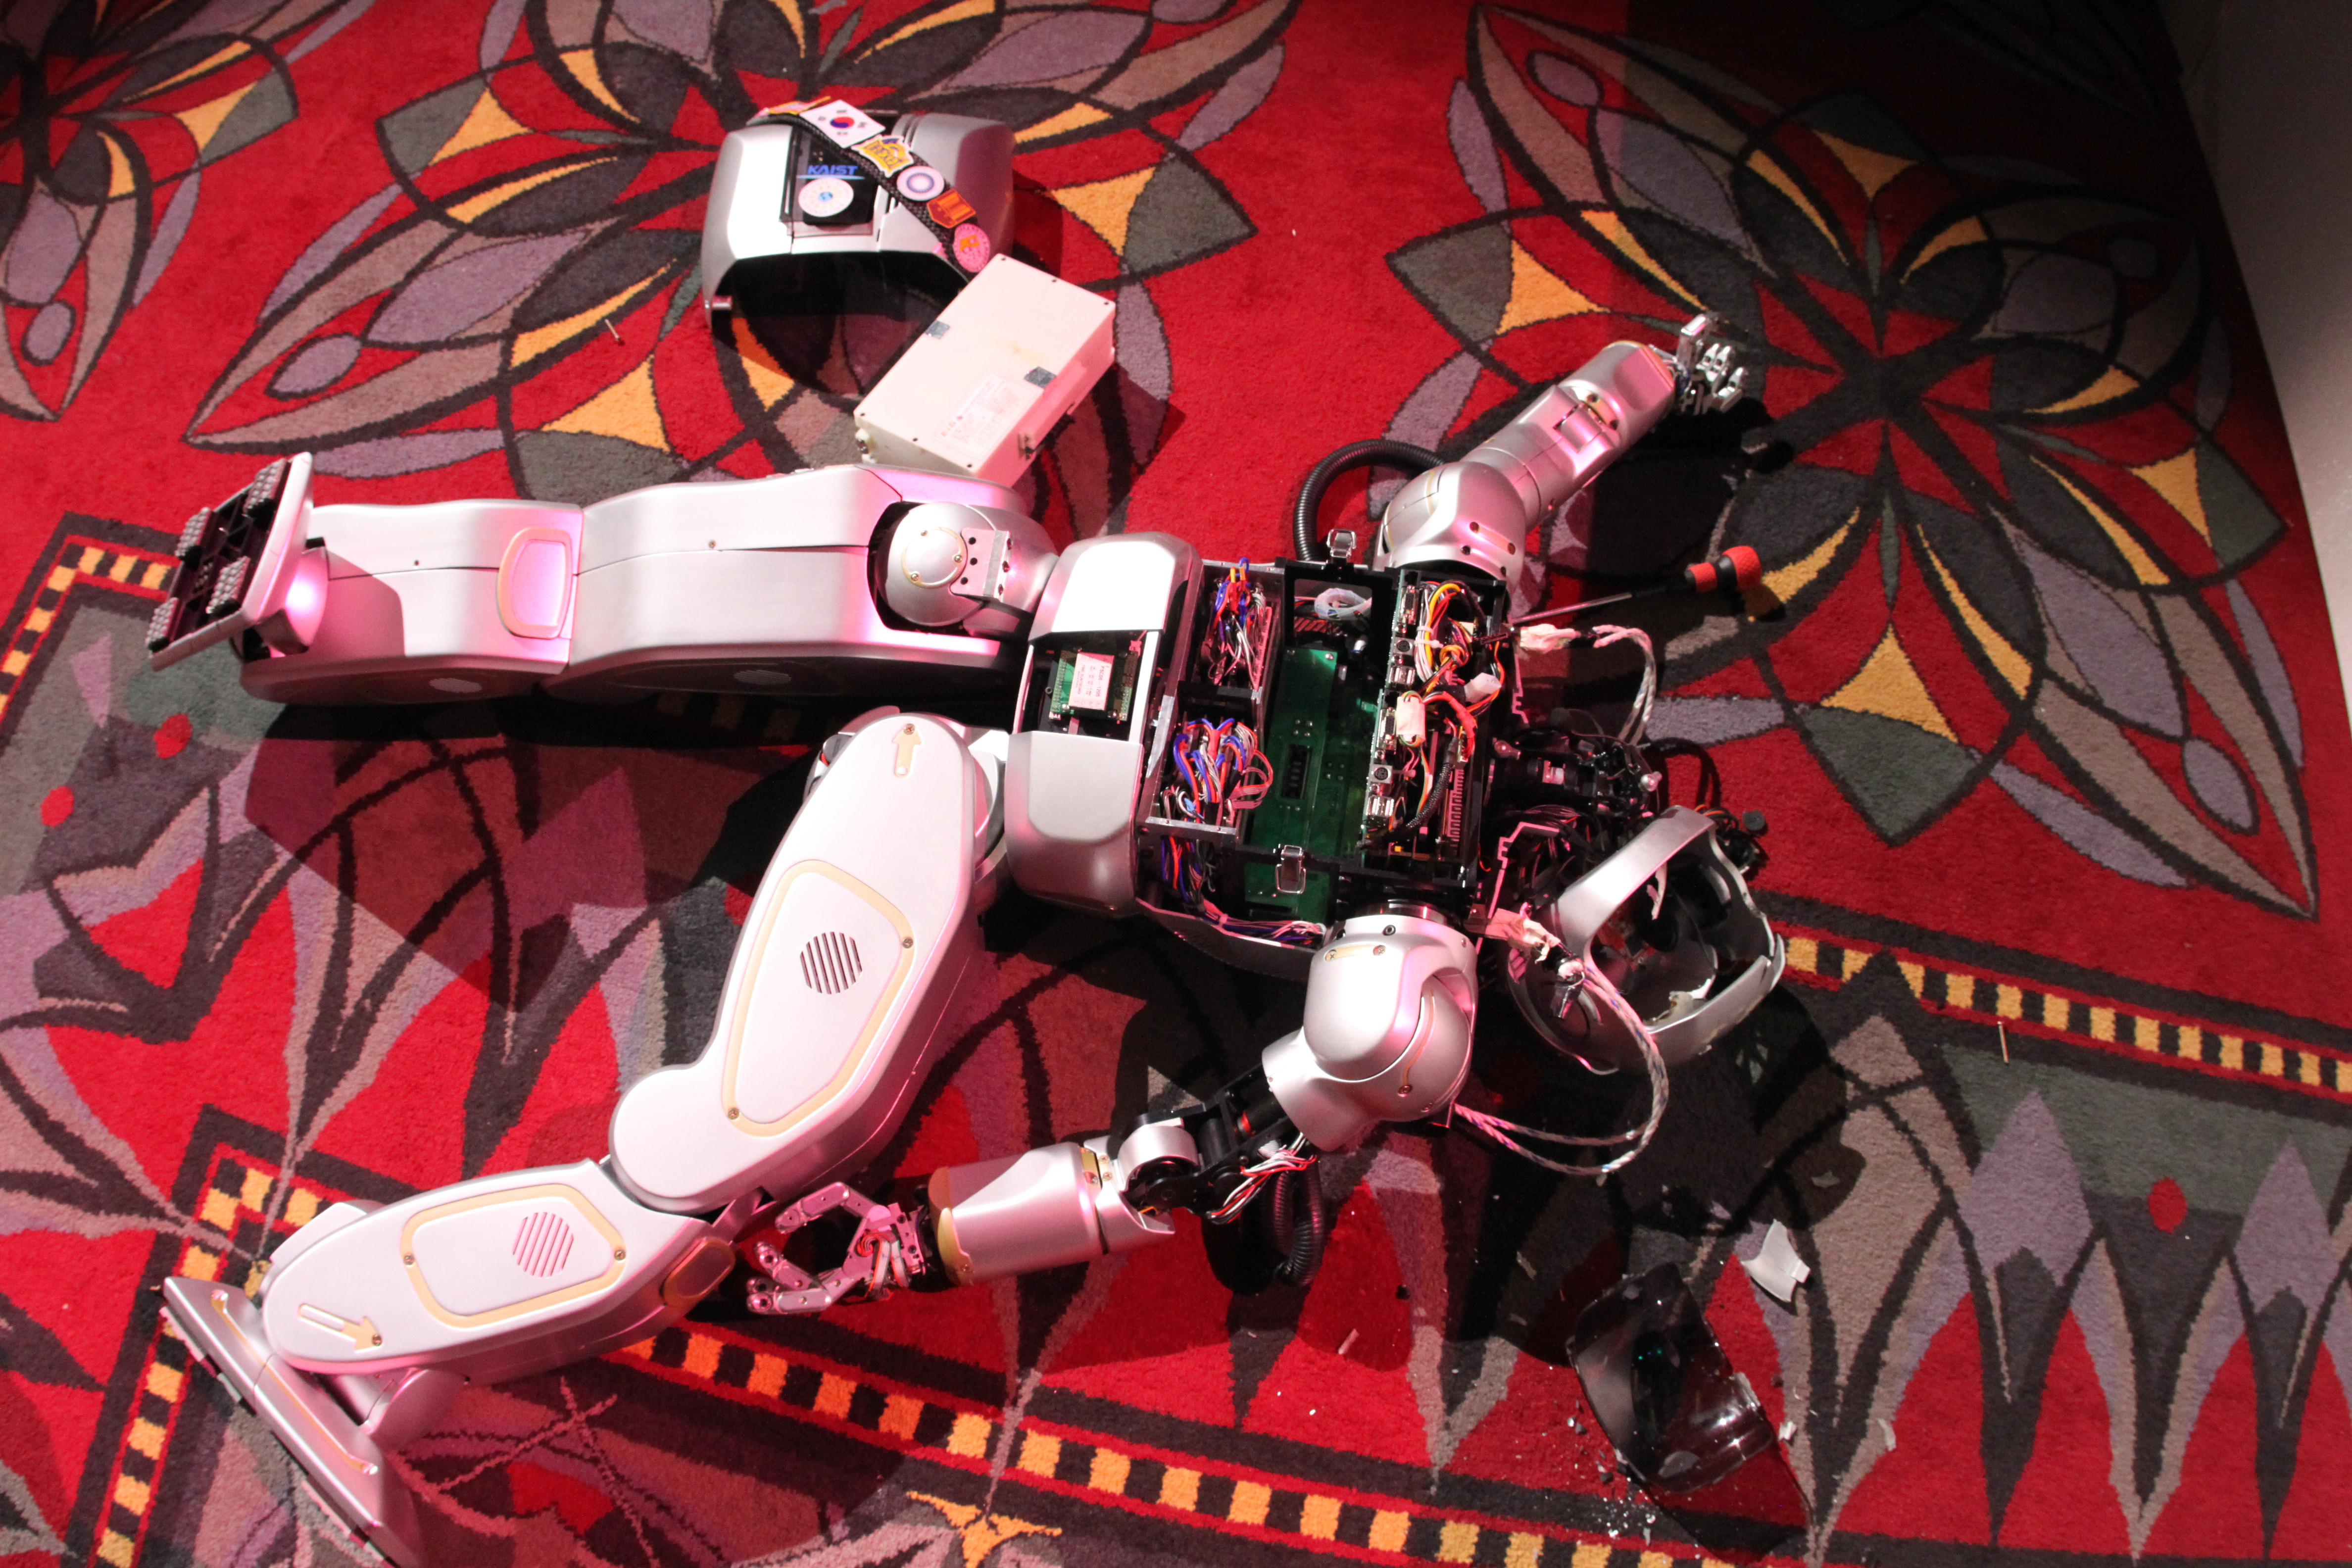
\includegraphics[width=1.0\columnwidth]{./pix/jaemiFall.png}
  \caption{Aftermath of the 4 foot fall Jaemi Hubo took after one of her actuators failed during operation.  A video with more images of the aftermath of the failure and further explanation of the event can be seen on YouTube.$^\ref{link:fall}$}
  \label{fig:fall}
\end{figure}  
 

Current methods of mitigation of ZMP loss for biped humanoids been investigated by Kiyoshi Fujiwara et al. \cite{4115653}.  These methods involve finding an optimal falling trajectory that reduces the instantaneous force of the robot at impact by creating multiple impact stages\cite{4399327}.  This method was fully tested on an HRP-2FX (HRP-2P surrogate) and partially on an HRP-2P.  This work did not include a method of determining a falling state, it is assumed that a fall is in progress.  Additional work on detecting a fall and reducing fall damage has been shown by Kunihiro Ogata et al.\cite{4755950}.  An active shok-reducing motion reduces the impact damage by following the center of gravity (COG) and attempting to keep it close to the ZMP support polygon.  The falling state is determined when the predicted ZMP departs from the support polygon. This method was tested on a miniature humanoid robot.  Additional work on determining a fall state using machine learning techniques\cite{4813885}.  Reimund Renner et al. used parameter estimation of multiple sensors to detect a falling state\cite{4058847}.

These methods are able to detect a specific fault state, however a need of detecting different fault states requires more general methods.  These methods must include monitoring not only sensor data but also actuator failure status.  